% didatic_example.tex — FED-HPC
%
% A two-job instance on which every one-pass greedy list-scheduling policy
% returns a schedule that is dominated by the exact weighted-sum optimum
% (model.solve_weighted_sum) for every lambda. Numbers verified with
% weighted_sum_reference, true_pareto_frontier, solve_weighted_sum and the
% baselines greedy_earliest_completion / threshold_bursting.
%
% Compile with:  latexmk -pdf didatic_example.tex

\documentclass[11pt,a4paper]{article}

\usepackage[margin=2.5cm]{geometry}
\usepackage[T1]{fontenc}
\usepackage{lmodern}
\usepackage{amsmath,amssymb}
\usepackage{booktabs}
\usepackage{tikz}
\usetikzlibrary{arrows.meta,positioning}
\usepackage{pgfplots}
\pgfplotsset{compat=1.18}
\usepackage{xcolor}
\usepackage{caption}
\usepackage[hidelinks]{hyperref}

\newcommand{\code}[1]{\texttt{#1}}
\newcommand{\fh}{\hat f}

\definecolor{jobA}{HTML}{4C78A8}
\definecolor{jobB}{HTML}{E45756}
\definecolor{deploy}{HTML}{BBBBBB}

% ------------------------------------------------------------ Gantt helpers --
% \gantt{content}: two rows (on-prem on top, cloud below), slots 0..8.
\newcommand{\gantt}[1]{%
\begin{tikzpicture}[x=0.68cm,y=0.75cm]
  \foreach \t in {0,...,8} {
    \draw[gray!40] (\t,-0.1) -- (\t,2.0);
    \node[below,font=\scriptsize] at (\t,-0.1) {\t};
  }
  \node[left,font=\small] at (0,1.5) {on-prem};
  \node[left,font=\small] at (0,0.5) {cloud};
  \draw[gray] (0,1) -- (8,1);
  #1
\end{tikzpicture}}
% \blk{row y}{start}{end}{colour}{label}
\newcommand{\blk}[5]{%
  \fill[#4,draw=black] (#2,#1+0.12) rectangle (#3,#1+0.88);
  \node[font=\small\bfseries,text=white] at ({(#2+#3)/2},#1+0.5) {#5};}
\newcommand{\dep}[2]{% deploy slot on the cloud row
  \fill[deploy,draw=black] (#1,0.12) rectangle (#2,0.88);
  \node[font=\scriptsize] at ({(#1+#2)/2},0.5) {$\pi$};}
\newcommand{\idle}[2]{% deliberately idle on-prem slot
  \fill[gray!15] (#1,1.12) rectangle (#2,1.88);
  \draw[dashed] (#1,1.12) rectangle (#2,1.88);
  \node[font=\scriptsize] at ({(#1+#2)/2},1.5) {idle};}

\title{A Didactic Example:\\ Why Greedy Misses the Weighted-Sum Optimum}
\author{FED-HPC}
\date{\today}

\begin{document}
\maketitle

\begin{abstract}
We build a two-job, two-type FED-HPC instance on which every one-pass greedy
list-scheduling rule (\code{greedy\_earliest\_completion},
\code{threshold\_bursting}, or a greedy that minimises each job's marginal
contribution to the weighted-sum objective) returns a schedule that is
\emph{Pareto-dominated}. The exact MIP (\code{model.solve\_weighted\_sum},
solved by Gurobi) finds a schedule that is better in \emph{both} turnaround and
cost. The key is a deliberately idle on-premises slot. A rule that commits
one job at a time, without looking ahead, can never choose it.
\end{abstract}

\section{Problem recap}

Each job $j$ has an arrival $a_j$, an execution time $e_j$ and an integer weight
$w_j$. It runs non-preemptively on one instance type $m$. That occupies
$p^{\mathrm{occ}}_{jm}=\lceil e_j/P_m+\pi_m\rceil$ slots (deploy $\pi_m$ is a time
penalty only) and costs $c_{jm}=\kappa^{\mathrm{VM}}_m\, e_j/P_m$. The on-premises
type has finite capacity; the cloud is elastic. The two objectives are
\[
  f_1=\sum_j w_j\,(C_j-a_j)\quad\text{(weighted turnaround)},\qquad
  f_2=\sum_j c_{j,m(j)}\quad\text{(cost)},
\]
and the weighted sum minimised by \code{solve\_weighted\_sum} is
\[
  \hat g_\lambda=\lambda\,\underbrace{\frac{f_1-f_1^T}{f_1^0-f_1^T}}_{\fh_1}
  +(1-\lambda)\,\underbrace{\frac{f_2-f_2^0}{f_2^T-f_2^0}}_{\fh_2},
  \qquad \text{s.t. } f_1\le f_1^0,\ f_2\le f_2^T,
\]
where $(f_1^T,f_2^T)$ is the lexicographic minimum-turnaround point and $f_1^0$
the minimum turnaround at the minimum cost $f_2^0$.

\section{The instance}

\begin{table}[h]
\centering
\begin{tabular}{lccc}
\toprule
Job & $a_j$ & $e_j$ & $w_j$ \\
\midrule
A (long, low priority) & 0 & 6 & 1 \\
B (short, urgent)      & 1 & 1 & 3 \\
\bottomrule
\end{tabular}
\hspace{1.5em}
\begin{tabular}{lccccc}
\toprule
Type & $N_m$ & $\pi_m$ & $\kappa^{\mathrm{VM}}_m$ & $p^{\mathrm{occ}}$ A\,/\,B & $c$ A\,/\,B \\
\midrule
on-prem & 1        & 0 & 0 & 6\,/\,1 & 0\,/\,0 \\
cloud   & $\infty$ & 1 & 1 & 7\,/\,2 & 6\,/\,1 \\
\bottomrule
\end{tabular}
\caption{Jobs (left) and instance types (right). Both types have $P_m=1$, no
I/O, and the horizon is $H=20$.}
\end{table}

\section{What greedy does}

A greedy list scheduler takes the jobs one at a time, in arrival order (or by
least slack, which gives the same order here). It commits each job to the best
start and type \emph{given the jobs already placed}, and it never delays a job
it could start now.

\begin{enumerate}
  \item At $t=0$ only A exists and the on-premises machine is free. Starting A
        there immediately is free and gives A its smallest turnaround (6,
        versus 7 on the cloud). Delaying A can only hurt A. Greedy commits
        A to on-prem $[0,6)$.
  \item At $t=1$ B arrives, but the machine is busy until $t=6$. Greedy can
        either
        \begin{itemize}
          \item \emph{queue} B on-prem $[6,7)$: $f_1=6+3\cdot 6=24$, $f_2=0$; or
          \item \emph{burst} B to the cloud $[1,3)$: $f_1=6+3\cdot2=12$, $f_2=1$.
        \end{itemize}
\end{enumerate}

\begin{figure}[h]
\centering
\begin{minipage}{0.48\linewidth}\centering
\gantt{\blk{1}{0}{6}{jobA}{A}\dep{1}{2}\blk{0}{2}{3}{jobB}{B}}\\[2pt]
\small Greedy, bursting: $(f_1,f_2)=(12,1)$
\end{minipage}\hfill
\begin{minipage}{0.48\linewidth}\centering
\gantt{\blk{1}{0}{6}{jobA}{A}\blk{1}{6}{7}{jobB}{B}}\\[2pt]
\small Greedy, queueing: $(f_1,f_2)=(24,0)$
\end{minipage}
\caption{The only two schedules a one-pass greedy can produce.}
\end{figure}

The repository baselines confirm this. \code{greedy\_earliest\_completion}
(with either ordering) and \code{threshold\_bursting} with $\theta\in\{0,3\}$
return $(12,1)$. \code{threshold\_bursting} with $\theta\ge 5$ returns $(24,0)$.
A ``weighted greedy'' that places each job where it adds the least to
$\hat g_\lambda$ also starts A at $t=0$ on-prem (contribution $6\lambda$ versus
$7\lambda+(1-\lambda)$). It then bursts B whenever $\lambda>1/73\approx0.014$,
again giving $(12,1)$.

\section{What Gurobi finds}

The exact Pareto front (\code{true\_pareto\_frontier}) has two points:

\begin{figure}[h]
\centering
\begin{minipage}{0.48\linewidth}\centering
\gantt{\idle{0}{1}\blk{1}{1}{2}{jobB}{B}\blk{1}{2}{8}{jobA}{A}}\\[2pt]
\small Hold the machine for B: $(f_1,f_2)=(11,0)$
\end{minipage}\hfill
\begin{minipage}{0.48\linewidth}\centering
\gantt{\blk{1}{1}{2}{jobB}{B}\dep{0}{1}\blk{0}{1}{7}{jobA}{A}}\\[2pt]
\small A to the cloud: $(f_1,f_2)=(10,6)$
\end{minipage}
\caption{The two Pareto-optimal schedules.}
\end{figure}

\begin{itemize}
  \item $(11,0)$: leave the on-prem machine \emph{idle} during $[0,1)$, run B
        in $[1,2)$, then A in $[2,8)$:
        $f_1=(8-0)\cdot1+(2-1)\cdot3=11$, at zero cost.
  \item $(10,6)$: run A on the cloud in $[0,7)$ and B on-prem in $[1,2)$:
        $f_1=7+3=10$, $f_2=6$.
\end{itemize}

The reference points are therefore $f_1^T=10$, $f_2^T=6$, $f_1^0=11$, $f_2^0=0$, and
\[
  \hat g_\lambda=\lambda\,(f_1-10)+(1-\lambda)\,\frac{f_2}{6}.
\]

\paragraph{Both greedy schedules are dominated.} The point $(11,0)$ is strictly
better than $(12,1)$ in both objectives and better than $(24,0)$ in
turnaround. So for \emph{every} $\lambda\in(0,1]$ the greedy schedule is
suboptimal. Greedy does not just pick the wrong trade-off; it is not on the
Pareto front at all. Both greedy schedules also violate $f_1\le f_1^0$, the
Pareto box that \code{solve\_weighted\_sum} enforces.

\begin{figure}[h]
\centering
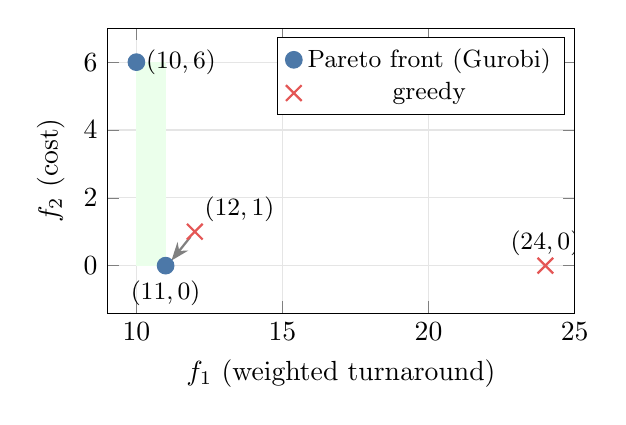
\begin{tikzpicture}
\begin{axis}[
  width=0.62\linewidth, height=5.2cm,
  xlabel={$f_1$ (weighted turnaround)}, ylabel={$f_2$ (cost)},
  xmin=9, xmax=25, ymin=-1.4, ymax=7,
  grid=major, grid style={gray!20},
  legend style={font=\small, at={(0.98,0.97)}, anchor=north east},
]
\fill[green!8] (axis cs:10,0) rectangle (axis cs:11,6);
\addplot[only marks, mark=*, mark size=3pt, color=jobA] coordinates {(10,6) (11,0)};
\addlegendentry{Pareto front (Gurobi)}
\addplot[only marks, mark=x, mark size=4pt, thick, color=jobB] coordinates {(12,1) (24,0)};
\addlegendentry{greedy}
\node[above right, font=\small] at (axis cs:12,1) {$(12,1)$};
\node[above, font=\small] at (axis cs:24,0) {$(24,0)$};
\node[below, font=\small] at (axis cs:11,-0.15) {$(11,0)$};
\node[right, font=\small] at (axis cs:10,6) {$(10,6)$};
\draw[-{Stealth}, thick, gray] (axis cs:11.85,0.85) -- (axis cs:11.2,0.15);
\end{axis}
\end{tikzpicture}
\caption{Objective space. The shaded box is the Pareto region $f_1\le f_1^0$,
$f_2\le f_2^T$. The arrow shows $(11,0)$ dominating the bursting greedy.}
\end{figure}

\begin{table}[h]
\centering
\begin{tabular}{cccccc}
\toprule
$\lambda$ & Gurobi schedule & $\hat g^\ast$ & greedy $(12,1)$ & greedy $(24,0)$ & gap of best greedy \\
\midrule
0.25 & $(11,0)$          & 0.250 & 0.625 & 3.50  & $+150\%$ \\
0.50 & $(10,6)$ or $(11,0)$ & 0.500 & 1.083 & 7.00 & $+117\%$ \\
0.75 & $(10,6)$          & 0.250 & 1.542 & 10.50 & $+517\%$ \\
\bottomrule
\end{tabular}
\caption{Normalised weighted-sum values. At $\lambda=0.5$ the two Pareto points
tie.}
\end{table}

\section{Why greedy fails}

The winning move, leaving the free machine idle during $[0,1)$, only pays off
because of B, and B has not arrived when A is placed. Seen from A alone, idling
is strictly worse: A's turnaround rises from 6 to 8. Any rule that scores one
job at a time against the jobs already placed rejects it, \emph{whatever the
score} (earliest completion, a bursting threshold, or the marginal
$\hat g_\lambda$).

This is the classic \emph{inserted idle time} phenomenon of scheduling with
release dates: non-delay schedules need not contain an optimum. The MIP picks
all start times $x_{jmt}$ at once, so it sees that holding the machine for one
slot buys B a turnaround of 1 instead of 2 or 6. With $w_B=3$, that is worth
more than A's two extra slots. The gap grows without bound as $w_B$ or $e_A$
increases: with $w_B=k$, the queueing greedy pays $f_1=6+6k$ against the
optimum's $8+k$.

\paragraph{Reproduce.} The instance is
\begin{center}\small
\code{Job(0,0,6,0,1,1,1,1)}, \quad \code{Job(1,1,1,0,1,1,1,3)}
\end{center}
with the two types above. Call \code{pareto.weighted\_sum\_reference},
\code{model.solve\_weighted\_sum},
\code{baselines.greedy\_earliest\_completion} and
\code{baselines.threshold\_bursting} to obtain every number in this document.

\end{document}
